





\section{What will we give up?}

So ends my speculation as to the manner in which collective prediction latches hold of your business. 

And I ask, what really stands between us and free artificial intelligence, given the topics we have visited thus far? The customary answer is privacy. Most readers may anticipate that the use of a tremendously powerful prediction utility is just another privacy trade-off - though I hope the just-so story hints at why this isn't the case.  

It's true that in this day and age we surrender a lot of our privacy in the name of convenience. We do this because other companies have scale, and the ability to use that data, and analytics, more effectively that we do. 

But I'm not going to make the argument that a common utility of immense power justifies a similar bargain. I'm sure there can be an element of that, but it mostly under-sells the potential. In this last chapter I have invited you to come at things from a different direction and ask if anything, really, needs to be given up. 
 
In fact there are a slew of techniques which you can use to avoid betraying commercial intent, surrendering data, or otherwise making a Faustian bargain. Some are very simple - so simple I won't discuss. 

But not everything is obvious. Mathematics has a lot to contribute to this conversation. We are on the cusp of a new age of privacy-preserving federated computation. Nobody doubts that. It is a reality. 

And all of the techniques that work in macroscopic ways (as with privacy-preserving consortia for medical records, to pick one) will also work in the small, in the tiny belly of the micro-manager. They are just algorithms, after all. 

The use of mathematics to protect privacy while preserving predictive power is not intuitive. It will take a while before the world (accustomed to identifying data with the predictive power of data, and accustomed to viewing private firms as separated by information barriers) unscrews its head and screws it on again backwards. 

So I'd say you have a good chance to get out in front. 

\section{A trade secret}

We'll get to what mathematics has to say momentarily, but first let's dive into an example where it might not be required. 

I'll pretend that you have a trade secret. Your trade secret is knowledge of a relationship between particulate matter in New York City ($X$) and same day equity returns ($Y$). You believe $X$ has a causal effect on $Y$ and you would like to leverage this knowledge without compromising your amazing discovery.

(Oops ... the impact of air pollution on stock prices has been studied in \cite{Levy2011AirUS} and \cite{Wu2018AirChina} among others.)

It's reasonable to ask whether use of a microprediction oracle that shoots your data into the public domain (there are safer kinds) can actually be useful to you. Will you not be giving away your interest in $X$, your interest in $Y$, or knowledge of their relationship? 
For now let's suppose we are brave souls performing naked public prediction. 

It isn't by any means a foregone conclusion that we'll mess up. I would say that it is a matter of technique. Rather than directly asking the oracle for predictions of recorded air pollution, $X$, you might instead ask an oracle to predict one or more quantities {\em caused} by $X$ - such as hospital admissions, recorded crime levels, the grammatical complexity in speech, performance on standardized tests, light sensor readings, temperature, solar electricity generation, or even bike-share trip durations.

You might be pleasantly surprised when the chain of micro-managers this gives rise to grows more complex over time, and when, eventually, particulate matter readings show up in the feature space. 

At this point, elsewhere in the web, predictions of particulate matter emerge - because as with our mosquito example from Chapter \ref{chapter:mental}, its always better to have forward looking predictions of regressors if you can find them (and as a consequence, almost everything in the web will be predicted). 

And so, in this manner, you have brought about the prediction of a quantity you care about, but with considerably reduced risk of anyone sniffing around your theory - since the prediction of particulate matter was initiated by someone else. 

Now maybe you get braver, flushed with success. And perhaps you try to be a little sneakier, too, and create a micro-manager where the compensation scheme is based not only on the accuracy of predicting hospital admissions, but on the predictive value of submitted data as it relates directly to stock returns - or something else you keep private. 


In doing so you make an entirely different discovery - one you never anticipated. You realize that in part, the relationship between $X$ and $Y$ can be partially explained away by a third variable $Z$ which appears to cause both. The realization has come to you with relatively little risk, and without the prediction web, you might never have arrived at this insight at all. 

\section{Structure preserving obfuscation}

Despite these possibilities, naked crowd-sourcing isn't for everyone. I'm going to consider far more defensive attitudes. 

One possibility is the use of transformations which disguise your data but preserve enough structure that outside algorithms can continue to help you. 

If the intent is mostly to source model insight, not data, and the machines on the other side of the oracle aren't going to try to interpret the data (merely predict it) there is little to be lost by transforming the data in a way that makes it unrecognizable but, at the same time, almost preserving of addition and multiplication. 

Because multiplication and addition are almost preserved, so are most things, hopefully, including linear algebra and machine learning techniques built upon that base.  

Going beyond obfuscation, strong encryption that preserves addition and multiplication is emerging from the labs at long last. It has been a journey since the surprising paper by Gentry in 2009 established the possibility.\endnote{\cite{Gentry2009AScheme}} 

A structure preserving transformation is called a homomorphism so the techniques are referred to as Homomorphic Encryption. Who can say how powerful they will be, a few years hence? I had no trouble locating $131$ papers on the subject published in the last three  months (Q1' 2021) alone.\endnote{ For a recent survey of homomorphic encryption see \cite{Alharbi2020SurveyTrend}} 

This approache comes with the drawback that other's might not be able to help you with exogenous data search - though you could arrange for that separately. This kind of two pronged approach is favored by hedge fund Numerai, for example, who separatedly crowd-source signals and algorithms.     

I suggest that in the context of using oracles {\em almost} homomorphic obfuscation will often be more than sufficient. It is not necessary to preserve all structure {\em precisely} when the objective is statistical prediction. Nor is it necessary to {\em completely} encrypt all data if the original reason for its protection falls short of the most sensitive categories. (Almost encrypted market data is not market data anymore, to pick one example).  

An example of a homomorphic transform is multiplication by your grandmother's age. Perhaps we throw in a rotation, or some portion of a neural network that has been trained to learn the identity mapping. The practical matter is that your ``data'', which might actually be model residuals, is often less than a military secret. 

It is entirely possible that you are accidentally, already performing a structure-almost-preserving pretty-good-obfuscation as part of your existing pipeline. 

\section{Algorithm preserving noise}

Adding noise in clever ways can help too, provided it does not defeat the purpose. It is becoming commonplace to see differential privacy employed when data is passed from one party to another. 


The idea is that an information budget is tracked, allowing a differential privacy layer to determine if individual record level information has been leaked over the course of numerous interrogations of the data. 

Unfortunately, what sometimes happens in practice is that the information budget is reset and new data introduced. This can defeat the ambition of keeping data private for a long period of time.

However in the fast flowing domain we care about, it is often the case that the commercial value of live data and its sensitivity degrades extremely quickly over time. So methods which only work for a limited time can be rather useful. 

And the research never stops. For every possible complaint we might raise about a given privacy preserving technique, there are no doubt several groups working to ameliorate it. For example, the use of local differential privacy may help with data sets that grow.\endnote{\cite{Joseph2020LocalData}} Differential privacy can be applied to algorithm results, not the data itself.\endnote{For a survey see \cite{Zhu2020MoreIntelligence} } 


\section{Those precious residuals}

I don't take privacy lightly, but I do expect it to fade in the minds of many as an obstacle to collective prediction. The key question might be whether everyone decides to send their model residuals to the micro-managers, or not. 

For as you will discern from the plausibility story that began this chapter, I predict that model residuals will be an important driver of prediction web adoption. 

There are some situations where residuals could betray intent, portfolio holdings, or something else - usually with simple workarounds. But for every one of these potential blunders there are a hundred situations where protection of model errors is precious, self-serving and disingenuous (if you really want to know how I feel about it) - aimed only at an attempt to prevent others from establishing the limitations of one's own modeling attempts.
 
Despite these comments, I will proceed as if the differences between your in-house model predictions and revealed ground truths are, in fact, the crown jewels. This helps us assess an ultra-defensive stance. 


Let's embed model residuals into a high dimensional space. The lagged values of any univariate time series can be considered a vector, as shown in Figure \ref{fig:residual}, where each coordinate is the value taken at a different time. The figure only represent three dimensions, of course. 


The time-series of your model residuals is the $\epsilon$ vector shown. The exogenous data can be represented on the same plot as well, and it is {\em likely} to be useful if it points in the same general direction as your data. I say that without too much loss of generality. Also, I am assuming that all your data is regularly sampled at the same times as your model residuals.


Putting these caveats aside, we have a ``Geometric Hypothesis of the Oracle Skeptic'' - one who declares that it is not possible to use microprediction oracles to improve your modeling, due to privacy concerns. 


Specifically, the skeptic will argue (I suppose) that an oracle cannot predict your residuals {\em unless} the actual residuals themselves are sent through that portal  - and that would be such a terrible thing, right? 

\begin{figure} 

\iftikz 
\makebox[\textwidth][l]{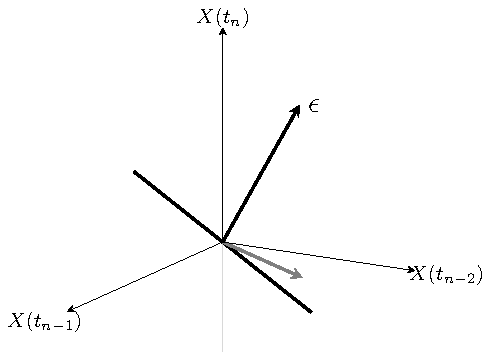
\includegraphics[width=0.6\textwidth]{09-privacy/PredictionWeb_tikz_privacy_geometry.pdf}}
\else 
\fi 
\caption{Model residual time series $\epsilon$ represented as a point in Euclidean space. Also shown is a grey vector that is very nearly orthogonal to the residuals, and thus not terribly useful.}
\label{fig:residual}
\end{figure}

Let us look to the outside world and ask if there is public data that can help us. Each of those time series can also be represented by a point in space but where are they? 


By definition of model residual, we have at our disposal only vectors that are mostly useless. An example is the grey vector in Figure \ref{fig:residual}. It is close to the hyperplane perpendicular to your data. For otherwise you would have included this data in your model, the hyperplane would move, and we'd be back to the start of the argument. 

\begin{figure} 
\scalebox{1.0}{
\iftikz 
\makebox[\textwidth][l]{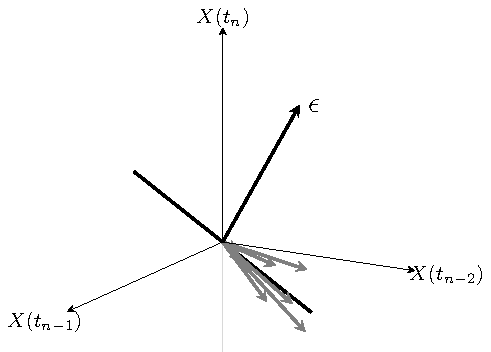
\includegraphics[width=0.6\textwidth]{09-privacy/PredictionWeb_tikz_privacy_geometry_2.pdf}}
\else 
\fi 
}
\caption{A collection of public data, and regressors for the same. Will it stay in the hyperplane perpendicular to the model residuals $\epsilon$?}
\label{fig:residual2}
\end{figure}

The skeptic finds it plausible that all the data is perpendicular. Let's set that aside and give them a pass, because the next question is tougher. Is it plausible that all the data that one might use to {\em predict all data in that plane} will {\em also} be perpendicular? What if we keep repeating? 


By starting with time series that were rejected predictors of $\epsilon$ (rejected at some level of significance, say) and then sourcing new data that predict {\em them}, and then new sources of data that predict those, and so on, we are going to have a tough time staying in the space orthogonal to $\epsilon$. 

Now we should be careful about making arguments in high dimensional spaces as our intuition is usually poor. It is also true that if $X \perp \epsilon$ then a predictor of $X$ is a lot less likely to be a good predictor of $\epsilon$ than a randomly chosen vector $X'$.  

Nonetheless, I think the prediction web and the relevance of its data to your predictions will sneak up on you. It's just a matter of time. 

As an aside this geometry helps us visualize the role of {\em weak universal data feeds} as noted in Section \ref{sec:universal}, and I would argue that the skeptic might require quite elaborate contortions to cling to their position.  

That's because one data feed can be used to create many {\em approximate} truths, including whether it is raining, windy or congested. By seeding other predictions, you encourage an eventual filling in of the space, as I noted in Chapter \ref{chapter:uses}.  


\section{The data lives of others}

I'm not sure if the preceding discussion will convince every hardened skeptic. After all, maybe your model residuals (or something causality related to them) are correlated with some other source of data - but that data is owned and kept private by someone else. 

You don't realize that. They don't realize that. The end?  

There are other versions of the same romantic tragedy. A vendor thinks they have data that is valuable to you. You suspect it is. But you cannot make a determination of this, and then effect a trade, without taking possession of the data. 


There are some traditional approaches to this last quandary, naturally, such as trial subscriptions, but they are far from perfect. The inability to know the predictive value of data is the old lemon's problem. The value of the data might lie in part in its historical record, so sometimes that can't be given up in advance of a trade. 


Other times the vendor can try to demonstrate value before the sale. But this too is problematic. The firm that might benefit from a new data source may be reluctant to reveal the intended use, and certainly not the model in which the data is used, as we have discussed. 

The inability to know the predictive value of other's data to you is one of the largest trade frictions. But there is another friction of trade which may be even more significant - though less apparent. 

I'd suggest that the real (perceived) ``problem'' with the trade of data is the fact that the seller of data thinks they need to provide the buyer with the data {\em after the sale}. If that sounds like a problem that cannot be solved, read on. 

I won't try to estimate the size of this problem, but of course we know that in recent times, sizable investments have been made by buy-side firms in predictive technology and data. There are more than one thousand companies that collect and sell alternative data to hedge funds, for example, over and above the existing enterprise data industry.\endnote{For a listing of alternative data vendors, see \cite{alternativedata}.} 


What if there was a way to discover a potentially mutually beneficial arrangement without the risk of revelation of commercially sensitive intent, or commercially valuable data? 

\section{Secret sharing}

We can couch this in a more general setting. Party A, Party B and Party C each possess data $a$, $b$ and $c$ that they have no intention of divulging to anyone. However all parties have an interest in learning the result of a calculation $f(a,b,c)$ that requires knowledge of all three data sets. 

A collection of devious methods for effecting this begin with Party A performing a random masking of data $a$ and a splitting of it into (say) three intertwined secrets $a_1, a_2$ and $a_3$. For example, if we suppose for simplicity that $a$ is an integer modulo $p=7$, then Party A can use a random number generator to produce $a_1, a_2$ and $a_3$ satisfying 
$$
       a_1 + a_2 + a_3 = a\ mod\ p 
$$
In a similar fashion, Parties B and C can also split their data into related secrets:
\begin{eqnarray*}
  b_1 + b_2 + b_3 & = &  b\ mod\ p \\
  c_1 + c_2 + c_3 & = &  c\ mod\ p 
\end{eqnarray*}
Party A now sends $a_3$ to Party C and sends $a_2$ to Party B, retaining $a_1$. Likewise, Party B sends $b_1$ and $b_3$ to Party A and Party C respectively, and finally Party C sends $c_1$ and $c_2$ to Party A and Party B respectively. 

This communication is yet to compromise the private number $a$ held by Party A, or likewise $b$ or $c$ held by Parties B and C respectively. Yet collectively, the information needed to reconstruct $a$, $b$ and $c$ exists in distributed form. 

In principle, depending on what the function $f(a,b,c)$ comprises, it {\em might} be possible to arrange for rounds of communication, and more secret passing such as this, that eventually arrives at the computation of $f(a,b,c)$. 

To prove this can sometimes be done, consider addition. More precisely, $f$ is the sum of the numbers $f(a,b,c)=a+b+c$ modulo $p$. Since this sum is also equal to the sum of all the distributed secrets by construction, it will be immediately revealed if all players add up the secrets currently in their possession and announce the answer to the other two parties! 

The question needs to be asked at this juncture: has anything been revealed that should not have been? The answer is no, though it requires careful checking. (For example, Party A is in possession of $b_1$ and $c_1$, and retained $a_1$ so she will announce $a_1+b_1+c_1$. But Party B can't do much with the number $a_1+b_1+c_1$.) 

There are also some weaknesses with the protocol. It requires all parties to honestly report, for example, and collusion amongst any two players is all it takes to leak information. 

Still, this simple example should immediately alter our mindset. Clearly, data is not the same as the use of data. There is immense potential of this rapidly moving field, known as secure multiparty computation. 

The reader might like to ponder how multiplication might be achieved. A clue is provide by the expansion
$$
   (b_1 + b_2 + b_3)(c_1 + c_2 + c_3) = b_1 c_1 + b_1 c_2 + \dots b_3 c_3 
$$
where it is observed that all terms require knowledge of two secrets only.\endnote{This introductory example of secret sharing, and the solution, is taken from  \cite{Cramer2015SecureSharing} where the reader may find a discussion of attacks, generalizations and applications.} Of course if we can achieve addition and multiplication, then many things follow - even gradient descent. 

Returning to our discussion of discovering the value of someone else's data, it is now clear that the computation of inner products in a secure manner can sniff out causal relationships, or at least suggest them. Here $f$ can be Granger causality, for instance. 

Furthermore, if $f$ is a machine learning model, then the use of an exogenous regressor in a prediction is not predicated on ownership of that data. Nor is it predicated on {\em revelation} of that data. The predictive power of data is completely divorced from the knowledge of the data itself. 

To me the the use of entangled secrets are reminiscent of quantum effects near the event horizon of a black hole. One photon from a pair passes through the horizon while the other escapes. In this prediction web analogy, even the most secretive of firms will, I predict, not be completely black. They will emit a kind of Hawking radiation.

\section{Luring adaptive algorithms} 
 
Perhaps in the future, as algorithms get smarter, firms will establish the AI equivalent of human resources departments. Therein, people and algorithms will be charged with attracting high quality adaptive algorithms to work on private data (inside their ``event horizons''). 

As with the human equivalent, the Artificial Resources department will assist the algorithms with this transition - making them comfortable and productive, and assuring them they are now part of the world's most exciting, open and ethically superior company in the whole of Northern California. 

But their real is recruiting. And that boils down to a privacy-hampered version of the race manager. A relatively easy problem, arguably, is the modification of that algorithm to work on internal systems, if we could somehow know in advance that it will work well. 

This is no different, in principle, to the problem of knowing whether a human candidate will perform well on a future task, given that it might not be appropriate to put them at the helm of a nuclear submarine immediately. Interview questions or other screening activities play the role of synthetic data - used to assess algorithms before they can see the real stuff.  

Synthetic data generation is problematic, admittedly, and a field unto itself. But even imperfect synthetic data can be a sufficient lure, one hopes, for adaptive algorithms capable of transferring {\em some} knowledge to unseen private data. In machine learning, the study of meta-learning, multitask algorithms, few-shot and transfer learning is proceeding at a break-neck pace. 

In the limit, as this generalized analytic ability improves, there will be no privacy issue at all. Data sensitivity issues only arise due to externalization of learning - for instance in a loop involving a human making occasional program updates. But if the algorithms are clean slates or do all the learning themselves, this isn't an issue. 


A possible solution involves a pair of race organizers. One of these micro-managers sits inside your firewall and has access to private data. The other sits outside, and does not. They run very similar contests.  


We presume that from time to time a small fraction of contestants in the external contest can be cloned, and transported inside the firewall where - unbeknownst to their authors - they will operate on private data {\em in addition to} the synthetic data used by the external micro-manager.  


Then, an iterative process can begin where ongoing refinements are made to the synthetic data used by the external micro-manager. That process can be informed by the relative performance of algorithms on the external versus internal data sets. Modifications to the synthetic data bring into closer alignment the ranking of algorithms in the external versus the internal leaderboards.  

I present this merely as an example of the kind of thing a human resources department for algorithms might do. Another idea is the design of testing sets that are calculated to fool algorithms that don't adapt - these test examples might be more extreme than the real world data, and cover more regimes.  

These tests can act like centrifuges, hopefully, separating out the algorithms that don't really have any special adaptive intelligence. Those that remain are more likely to assist in tasks their authors are yet to see. 


\section{Keeping it simple}

I close by tabulating some approaches to privacy preservation that are mostly self-explanatory. It would be foolhardy to suggest there is one best way to address risk, regulatory or other concerns. For one thing, there isn't one concern. Are you concerned about theft? What about piracy? 

Contamination of the data with a small number of erroneous data points (ignored by scoring rules) may deter unpaid commercial usage. Steganography can be used to make statistically insignificant yet traceable changes to the data, enabling a subsequent investigation to identify the precise participant who was the source of the stolen goods. 

There are too many approaches to give names to, at least standard ones, but Table \ref{tab:datause} enumerates some issues and countermeasures. Some we have discussed. Others are self-evident. And some, like the use of contracts, are too obvious to even include in the table. 

It's worth noting that many of the concerns regarding microprediction also apply to alternative data, and that hasn't stopped that area from exploding in recent years.  

\begin{table}
\begin{tabular}{|l|l|l|}
\hline 
  Concern  & Example              &  Techniques    \\ \hline
  Intent & Sensitive targets & Weak truths \\ 
         &            & Residuals \\ 
         &            & (and many below) \\ \hline
  Theft    & Subscription data & Sub-sampling, \\ 
                  &                 & Contamination,              \\
                  & .               & Dilution, \\
                  &                 & Blacklisting,           \\
                             &                 & (and all below)     \\
  \hline
 Piracy   & Reselling   &  Steganography, \\
                   &                      & Bootstrapping, \\
                   &                      & Transformation \\
                             &                 & (and all below)     \\
         \hline
  Privacy  & Proprietary data   &  Allowed-list,   \\  
         &                               & Private contests  \\
         &                               & Obfuscation  \\
         &                               & Differential privacy \\
                             &                 & (and all below)     \\
         \hline
  Secrecy & Classified data      & Chumming \\
           &                     & Multi-party computation   \\
           &                     & Structure preserving encryption  \\
           &                     & Centrifuge \\
   \hline
\end{tabular}
\caption{Defenses against misuse of data supplied to participants (or not supplied as the case may be).}
\label{tab:datause}
\end{table}



\section{Summary}

Privacy and intellectual property are important. However, they do not preclude the growth of a microprediction web within and between private firms. Many sensible steps that can be taken to avoid leaking commercial intent or intellectual property. 


To grow, a microprediction web needs only to add value by leveraging the {\em predictive power of data} which may be possessed and guarded closely by separate parties. But fortunately, this does not require those parties to reveal their data to each other. 

Skepticism of collective prediction is understandable, but {\em predictive ability} will flow freely between firms much more effectively than it has in the past - even if private raw data stays where it should. Indeed a network of micro-managers is precisely what we need to infect the world with privacy-preserving mathematics. 

So, I close by suggesting that an effective way to visualize the potential for a microprediction network is to imagine that boundaries between firms do not exist at all. 



